\chapter{基于传统机器学习方法的低分辨率环境下微表情识别}\label{chap:owner1}

微表情属于常规性非言语行为,可以真实的表达人类隐藏的情感。它在国家安全、计算机辅助医疗等领域有着非常广泛的应用,这鼓励我们开展微表情自动识别的研究。然而,从监控视频中获取的图像容易出现质量低下等问题,给实际应用带来非常大的困难,使得所有研究都只能在实验层面。由于通过监控视频所捕获图像的质量较低,现有的算法无法达到预期的效果。针对这一问题,我们对低分辨率情况下模糊人脸的微表情识别问题进行了全面的研究并提出了完整的低分辨率环境下微表情识别框架。实验结果表明,该框架在低分辨率情况下的微表情识别中取得了优异的成果。

目前常规的微表情识别算法虽然取得了良好的识别效果,但其性能在很大程度上取决于人脸视频片段的质量。一旦用于识别的人脸视频片段质量较差(如分辨率较低),章节\ref{chap:relate}中提及的算法就无法正常工作。原因主要在两个方面:(1)低分辨率图像丢失了大量的纹理信息,导致从低分辨率图像序列中提取可用特征变的困难\citep{lei2011local}。(2)低分辨率图像与高分辨率图像质量(不同分辨率、不同清晰度)不一致,导致我们在测试阶段无法直接使用低分辨率图像作为输入。同时,当处于真实环境时,从监控录像中获取的人脸图像通常只占整个画面的一小部分,例如,用于微表情识别的SMIC数据集的人脸分辨率为$190\times230$(SMIC数据集的分辨率为$640\times480$)。然而更严重的是,常规监控视频捕捉到的图像序列的人脸分辨率往往在$50\times50$(或更低)以下。这意味着之前的微表情识别方法不能直接用于处理低分辨率的情况。因此,对低分辨率环境下的微表情识别的研究具有重要意义和挑战性。

\begin{figure}[!htbp]
    \centering
    \includegraphics[width=0.98\textwidth]{LR0}
    \caption{低分辨率环境下微表情识别框架}
    \label{fig10}
\end{figure}

为了解决上述问题,我们利用最新的人脸Hallucination方法进行了低分辨率微表情识别的研究。我们首先对低质量的人脸图像序列Hallucination处理,以近似的重建出丢失的动态特征。然后,我们再采用传统的微表情识别算法识别低质量的微表情图像序列。我们评估了不同分辨率下微表情识别的准确率,研究了分辨率与识别准确率之间的关系。总的来说,本章的目的是全面研究分辨率对微表情识别的影响,同时提出一个基于传统机器学习方法的处理低质量条件下微表情识别任务的框架。

如图~\ref{fig10}所示,低分辨率微表情识别过程包括图像序列预处理、超分辨率重建、特征提取和分类。详细内容将在本章的以下部分展开描述:

\section{低分辨率微表情数据获取}

目前常用的微表情识别的数据集有很多,如SMIC和CASME等。然而,这些数据集都是专业相机在严苛环境下获取的高清图像序列,表~\ref{tab3}详细描述了各数据集的参数。图~\ref{fig11}列举了SMIC-HS数据集中一个视频片段中的两帧。我们可以在红色框的范围中发现面部表情的细微变化,特别是白色椭圆区域和白色箭头指向的位置运动更为明显。然而,如果图像质量过低,这些细节很难被注意到。

\begin{figure}[!htbp]
\centering
\includegraphics[width=0.65\textwidth]{LR1}
\caption{来自SMIC-HS数据集的两帧}
\label{fig11}
\end{figure}

由于现有的自发微表情数据集中不存在低分辨率的图像序列,所以我们采用图像退化处理的方法来获得模拟的低分辨率微表情图像序列。论文\citepns{wang2014low}将低分辨率图像分为三大类:小尺寸(Small Size)、低质量(Poor Quality)和小尺寸\&低质量(Small Size \& Poor Quality)。我们考虑第三种类型的图像(小尺寸\&低质量)作为模拟图像,这样更接近真实应用的情况。

在图像重建任务中,低分辨率图像序列是通过对高分辨率图像序列进行模糊、下采样和噪声处理得到的\citep{shi2018hallucinating},如下式所示:
\begin{equation}
    \label{eq1}
    \boldsymbol{L} = \boldsymbol{DBH}+\boldsymbol{n}
\end{equation}
其中 $\boldsymbol{D}$和$\boldsymbol{B}$分别是下采样和模糊处理,$\boldsymbol{H}$是高分辨率图像,$\boldsymbol{n}$是加性噪声,$\boldsymbol{L}$是低分辨率图像。我们按照公式~\ref{eq1}的原理对原始数据处理获得实验所需的低分辨率微表情数据,具体如章节\ref{exp}的实验部分所示。

\section{数据预处理}

在我们提出的框架中,预处理主要包括三个步骤:人脸对齐、人脸分割和帧插值处理。原始视频中存在自然的姿势变化和无意识的移动,数据集中收集了不同性别、年龄和种族的参与者的微表情视频片段。因此,为了避免上述非表达因素的干扰,进行人脸对齐和人脸分割是必不可少的。同时,由于微表情的强度是非常微弱的,为了减少类内变化和突出微表情运动产生的类间差异,更需要最小化微表情片段间的其他差异(如人脸大小和人脸形状)。为此,我们使用以下描述方式对所有人脸与模型脸对齐处理。

首先,我们选择一个中性的人脸图像作为模型人脸,使用主动形状模型检测模型脸的68个人脸关键点,接着对第$i$个微表情片段的第一帧上的人脸检测68个关键点,然后使用局部加权平均计算它们之间的关系,对微表情片段的所有帧均使用上述关系进行归一化。最后,将归一化后的图像换算为原始图像的二维变换,根据第一帧中瞳孔的坐标,从每个微表情片段的归一化图像中裁剪出人脸区域。详细过程如下文所示:

\subsection{主动形状模型}

从采集的视频中选取其中没有表情且正面人脸的一帧作为模型脸$\boldsymbol{I_{mod}}$ ,手工定位两只眼睛的位置。然后,利用主动形状模型(Active Shape Model, ASM)检测68个人脸关键点$\boldsymbol{\psi(I_{mod})}$\citep{cootes1995active}。值得注意的是,传统的ASM算法机械地通过检测差异点获取目标,并没有选择目标对错的能力,本章在原算法的基础上增加了条件限定,使得检测的人脸更加准确、规范。如错误标定其他物品或其他人脸(非主要人脸)时,计算任意对应位置关键点的相对距离$\boldsymbol{L(I_{mod})}$ :
\begin{equation}
    \label{eq2}
    \boldsymbol{L^{(i)}(I_{mod})}=\left \| \boldsymbol{\psi_{I_{mod}}}(p\pm 68)-\boldsymbol{\psi_{I_{mod}}}(q\pm 68) \right \|_{2}^{2\displaystyle }
\end{equation}
其中$i$指标定的关键点组数,$p$、$q$指一个关键点组中任意两点,$n$为关键点的个数,数量为68的倍数。选择相对距离$\boldsymbol{L^{(i)}(I_{mod})}$ 最大的一组关键点来确定视频帧中主要人脸。如图~\ref{fig12}所示,1框内为目标人脸,2框为错误识别。通过上述算法在实验过程中错误标定率明显下降。

\begin{figure}[!htbp]
\centering
\includegraphics[width=0.70\textwidth]{3LR1}
\caption{ASM算法标定的68个人脸关键点}
\label{fig12}
\end{figure}

\subsection{局部加权平均算法}

对每段个视频的第一帧$\boldsymbol{I_{j,1}}$应用ASM算法标定68个人脸关键点$\boldsymbol{\psi (I_{j,1})}$,使用局部加权平均函数(Local Weighted Mean,LWM)建立模型脸关键点集$\boldsymbol{\psi (I_{mod})}$与视频第一帧关键点集$\boldsymbol{\psi (I_{j,1})}$之间的对应关系\citep{goshtasby1988image}:
\begin{equation}
    \label{eq3}
    \boldsymbol{T_{j}}=LWM(\boldsymbol{\psi (I_{mod})},\boldsymbol{\psi (I_{J,1}))},~~j=1,\cdots ,l
\end{equation}
其中$j$是视频段号,$l$是视频片段总数。对视频片段的所有帧应用该关系,使视频的每一帧具有与模型脸$\boldsymbol{\psi (I_{mod})}$统一的姿态:
\begin{equation}
    \label{eq4}
    \boldsymbol{I_{j,k}^{'}}=\boldsymbol{T_{j}}\times \boldsymbol{I_{j,k}},\quad k=1,\cdots ,n_{j}
\end{equation}
其中$\boldsymbol{I_{j,k}}$为第$j$个视频片段的第$k$帧,$\boldsymbol{I_{j,k}^{'}}$为统一姿态后的第$j$个视频片段的第$k$帧,$n_{j}$为$j$视频片段的帧数。如图~\ref{fig13}所示,两图均按照模型脸统一姿态,左图剔除了错误识别,右图改变了头部的倾斜角度,实验表明通过这种方法大大减少了非表情因素的干扰。

\begin{figure}[!htbp]
\centering
\includegraphics[width=0.70\textwidth]{3LR2}
\caption{LWM算法人脸对齐后的图像}
\label{fig13}
\end{figure}

\subsection{时间插值模型}

微表情识别其中一个特殊的挑战是微表情持续时间短。例如,SMIC数据集中最短的片段持续时间为3/25秒,只有3帧(25 fps)之多。这样的短序列严重限制了许多时空特征描述符的应用,如LBP-TOP特征沿时间维度的可行半径$r$只能为1。除此之外,微表情视频片段之间有不同的长度,而且变化也相当大,从4帧到50帧(如果用100帧/秒的相机拍摄)不等,这也对一些对视频帧数敏感的特征描述符提出了挑战。

Zhou等人在论文\citepns{zhou2011towards}中提出了一种时间插值模型(Temporal Interpolation Model,TIM)。该模型在原论文中用于唇语识别(Lipreading),论文中提到如果我们将一段视频中讲话嘴的运动视为连续过程,则语音视频的图像序列可以被视为沿着表示图像空间中话语的曲线以固定速度采样的一组图像,或更一般地表示为从图像中提取的视觉特征。通常,这样的空间具有高维度,并且我们可以假定存在一个低维流行,其中连续的发声过程可以通过连续和某种确定性函数来表征。根据这样的特性,我们将其一般化地应用到低分辨率环境下微表情识别的框架中,使用TIM方法来解决与微表情持续时间和帧数差异相关的问题。在我们的工作中,我们通过将输入视频表示为路径图$P_{n}$来揭示这样的功能,其中$n$是顶点数。图~\ref{fig14}(a)给出了这种图表示例,如图所示,每个顶点对应于一个帧,并且顶点之间的连接可以由邻接矩阵$\boldsymbol{W}\in \left \{ 0,1 \right \}^{n\times n}$ 表示,其中当$\left | i-j \right |= 1,~ i,j=1,2,\cdots ,n$时$W_{ij}= 1$,否则为0。

\begin{figure}[!htbp]
    \centering
    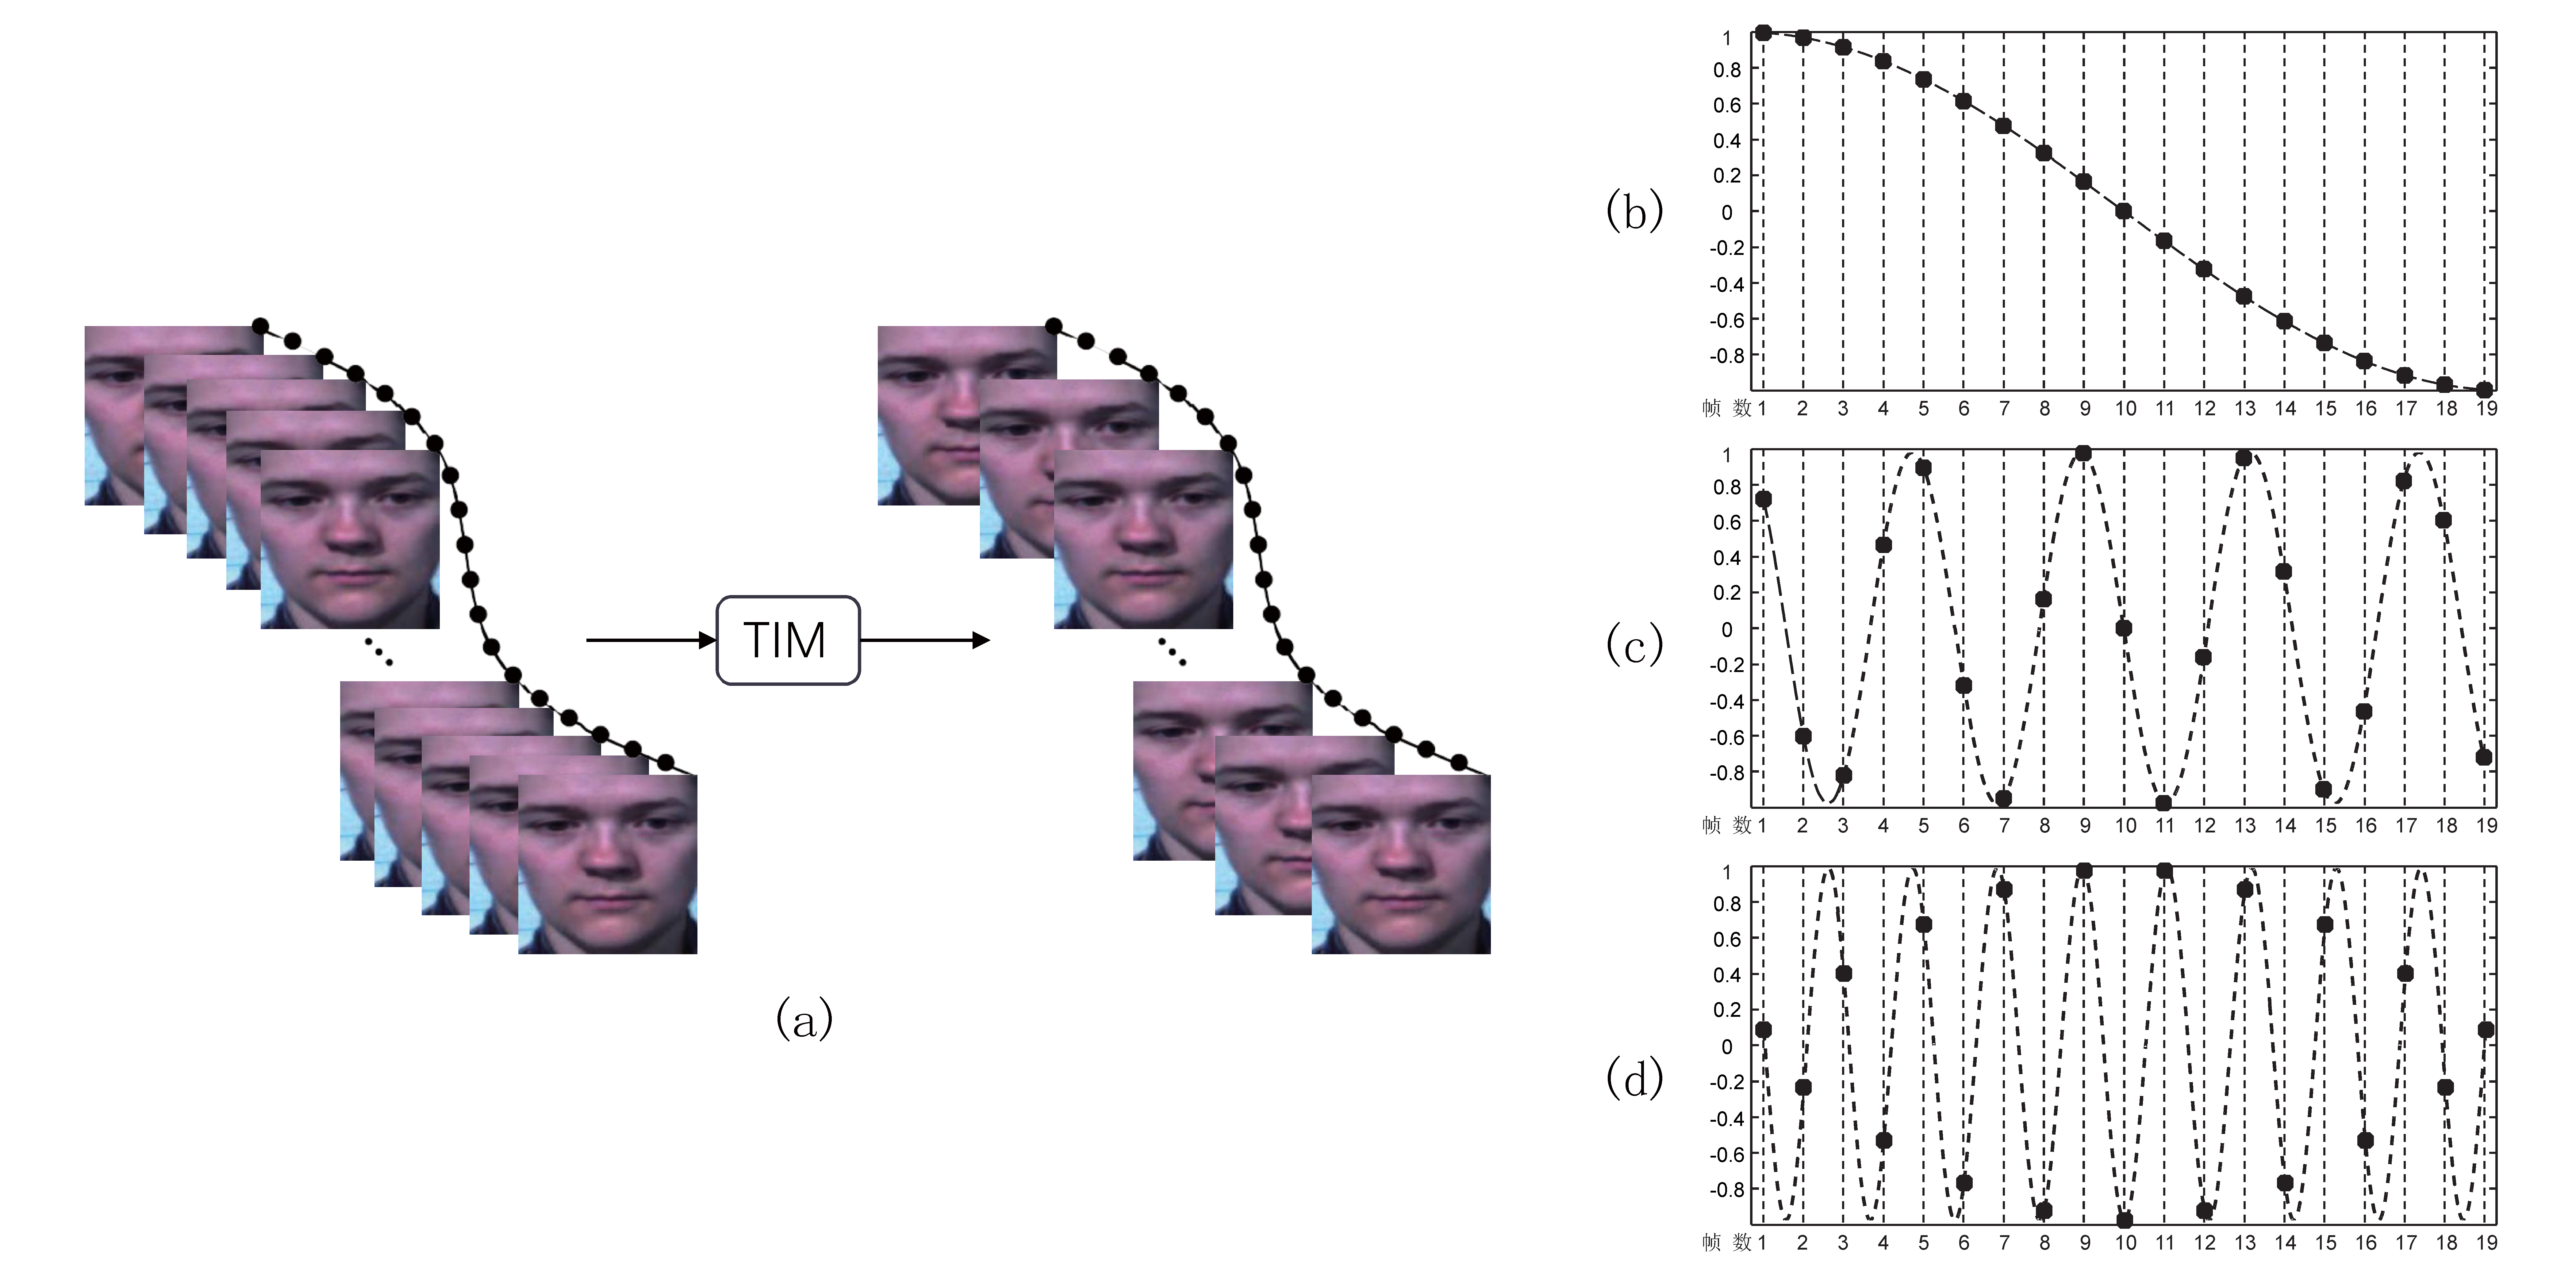
\includegraphics[width=0.9\textwidth]{LR2}
    \begin{spacing}{1.0}
    \caption{TIM方法映射过程}
    \label{fig14}
    \centerline{\footnotesize \textmd{(a)共19帧的图像序列插值过程($P_{19}$ ),输入为原始图像,输出为插值后图像;}}
    \centerline{\footnotesize \textmd{(b)-(d)为图像序列的Laplacian第1、第9和第18特征向量的映射。}}
    \end{spacing}
\end{figure}

在本文中对由重建出的高分辨率图像组成的图像序列应用TIM算法统一帧数:将重建的图像序列映射到一条非线性曲线上$\mathcal{F}^{n}:\left [ 1/n,1 \right ]\rightarrow \mathbb{R}^{n-1}$ ,
\begin{equation}
    \label{eq5}
    \mathcal{F}^{n}(t)=\begin{bmatrix}f_{1}^{n}(t)\\ f_{2}^{n}(t)\\ \vdots \\ f_{n-1}^{n}(t)\end{bmatrix}
\end{equation}
其中$f_{k}^{n}(t)=sin(\pi kt+\pi (n-k)/n),\quad t\in \left [ 1/n,1 \right ]$ ,$n$为视频段中帧数(图像序列个数),根据实验需求等间距采样,获得统一帧数。

TIM方法通过路径图来描述帧序列的结构:学习图像序列特定的映射以连接图像序列中的帧和嵌入在路径图中的曲线,从而将图像序列投影到路径图中,如图~\ref{fig14}(a)所示。图~\ref{fig14}(b)-(d)的曲线是[0,1]区间内单个变量$t$的连续确定性函数,控制着帧间的时间关系。在微表情的连续过程中出现的不可见的帧也可以用曲线来表征。因此,使用TIM方法,无论是向下采样还是向上采样,通过控制变量$t$在不同时间点的变化,我们都可以将帧序列改变为任意长度。

在本文提出的框架中,TIM方法被用来将所有的微表情片段(数据集)插为一个固定的长度,例如,10帧、20帧或40帧。这样既可以解决持续时间短的问题,也可以解决序列长度不统一的问题。当前步骤的目的一方面可以在选择特征参数时提供更多的选项,另一方面利用时空特征描述符实现更稳定的性能。如何选择最合适的TIM插值长度的问题在论文\citepns{Li2017Towards}中进行了探讨和讨论,本文将其讨论结果作为参考,具体如章节\ref{exp}的实验部分所述。

\section{超分辨重建过程}

在本文中,我们分别提出了基于块和基于像素的两种新的正则化,它们可以有效地将输入的低分辨率人脸图像重建成高分辨率人脸图像。与依赖于低分辨率和高分辨率空间中局部几何一致性假设的传统基于块的模型不同,所提出的方法直接规范了目标块与高分辨率空间中相应训练集之间的关系。它避免了处理在不同分辨率下保留局部几何结构的棘手问题。利用核函数有效地描述内在特征,我们在高维核空间进一步进行基于块的模型重建,以捕获非线性特征。同时,提出了一种基于像素的模型来规范局部邻域中像素的关系,可以用来增强目标高分辨率人脸图像中的模糊细节。它主要是沿着结构的主导方向重建像素,这对于保留复杂边缘上的高频信息是有用的。最后,我们将两个重建模型组合成一个统一的框架。可以通过执行迭代过程来最终优化输出重建的高分辨率人脸图像。实验结果表明,所提出的人脸Hallucination方法比现有技术方法具有更好的性能。

重建模型$\mathbf{L=DBH}+\varepsilon$ 中的高分辨率人脸图像$\mathbf{H}$严重欠定,意味着每个低分辨率人脸图像对应于无限多个高分辨率估计。为了改善这个问题,必须在整个重建过程之前加入进一步的正则化。通过附加先验条件,可以获得高分辨率人脸图像$\mathbf{H}$的唯一解决方案。重建模型可以表示为:
\begin{equation}
    \label{eq6}
    \mathbf{H} = \mathrm{arg}~\underset{\mathbf{H}}{\mathrm{min}}\left \{ \left \| \mathbf{L-DBH} \right \| _{2}^{2}+\gamma R(\mathbf{H}) \right \}
\end{equation}
其中$R(\mathbf{H})$表示正则化模型,$\gamma$是平衡重建误差和正则化项的相应参数。在\ref{eq6}中,第一项确保了估计的高分辨率人脸图像和观察到的低分辨率人脸图像的一致性,而附加的先验项进一步规范了高分辨率人脸图像的局部细节。根据人脸图像的特点,提出了两种有效的正则化模型,以约束重建过程。以下将描述上述两个先验项的细节。

低分辨率图像和高分辨率图像在质量和分辨率上都是不同的。高分辨率图像序列的微表情识别方法不能直接应用于低分辨率图像序列。在2.1节中,我们介绍了从高分辨率图像生成低分辨率图像的过程。

为了重建高分辨率图像,论文\citepns{shi2018hallucinating}提出了一种新的人脸幻觉算法。将基于块的正则化项与基于像素的正则化项相结合,对目标函数进行约束。重构后的高分辨率图像$\boldsymbol{H}$可以通过最小化以下目标函数得到:
\begin{equation}
 \label{eq7}
 \begin{split}
    f\left ( \boldsymbol{H} \right )= \left \| \boldsymbol{L}-\boldsymbol{DBH} \right \|{_{2}^{2}}+\alpha \boldsymbol{F}_{patch}+\eta \boldsymbol{F}_{pixel}+\lambda \boldsymbol{F}_{penalty}
 \end{split}
\end{equation}
其中右侧第一项为重建误差,后三项分别是基于块的正则项、基于像素的正则项以及惩罚项。图~\ref{fig15}展现了重建工作的具体流程。具体将在下文详细介绍。

\begin{figure}[!htbp]
\centering
\includegraphics[width=0.75\textwidth]{LR3}
\caption{超分辨重建过程}
\label{fig15}
\end{figure}

\subsection{基于的块方法}

将分割后的图像$\boldsymbol{L}$(低分辨率图像)应用三线性插值法调整为与训练样本图像$\boldsymbol{H}$(高分辨率图像,来自公开的高分辨率图像集)大小相等的尺寸,将此图命为$\boldsymbol{H^{(0)}}$(超分辨重建过程的初始图像),对图像分块处理(如分块数为$8\times8$),如图7所示,最小化代价函数:
\begin{equation}
 \label{eq8}
 \begin{split}
   \boldsymbol{J_{\tau }(\omega _{\tau },H^{(k)})} & =\left \{ \left \| \boldsymbol{\phi (R_{\tau }H^{k})}-\boldsymbol{\phi (H_{\tau })\omega _{\tau }} \right \| _{2}^{2}+\boldsymbol{\lambda} \left \| \boldsymbol{d_{\tau }}\bigotimes \boldsymbol{\omega _{\tau }} \right \|_{2}^{2}\right \} \\
   \boldsymbol{s.t. 1^{T}\omega _{\tau }}= 1 & ,2,\cdots ,M
 \end{split}
\end{equation}
估算结合系数$\boldsymbol{\omega _{\tau }}$ ,将其初始结合系数命名为$\boldsymbol{\omega_{\tau }^{0}}$,此时$\boldsymbol{H^{(k)}}$ 已知,即$\boldsymbol{H^{(0)}}$ ,其中$\boldsymbol{\tau}$为图像中图像块的位置,$\boldsymbol{R_{\tau }}$为提取所有图像集位置$\tau$的图像块的矩阵, $\boldsymbol{H_{\tau }}=\left [ h_{\tau }^{1},\cdots ,h_{\tau }^{N} \right ]$为高分辨率图像位置$\boldsymbol{\tau}$处图像块集($N$为训练样本的数量,即高分辨率图像集的数量),$\boldsymbol{\phi (\cdot )}$ 为从原始空间到无限维再生核希尔伯特空间(Reproducing Kernel Hilbert Space, RKHS)的映射,$\boldsymbol{d_{p}}$ 描述了目标高分辨率块(重建出的块)与相应的训练样本块在核映射空间的核相似性,$\bigotimes$ 表示哈达玛积,$\boldsymbol{\lambda}$为惩罚系数,$\boldsymbol{1}$为全为1的列向量,$M$为图像的块数。

\subsection{基于像素的方法}

可以通过解决上述优化问题(25)来获得最终的高分辨率人脸图像$\boldsymbol{H}$。但是,目标函数是非凸优化问题,很难直接获得全局最优解。幸运的是,我们可以期望通过迭代过程获得局部最优解。为了解决(25)中的问题,我们可以分别优化$\omega _{\tau }$和$\boldsymbol{H}$,同时固定另一个值。例如,如果$\omega _{\tau }$的值是固定的,则可以通过最小化以下函数来获得最优$\boldsymbol{H}$:
\begin{equation}
 \label{eq9}
 \begin{split}
   \boldsymbol{f(H)}= \left \| \boldsymbol{L^{k}}-\boldsymbol{DBH^{k}} \right \|_{2}^{2}+\boldsymbol{\eta \sum_{\tau }}\left \| \boldsymbol{x_{\tau }h^{k}}-\boldsymbol{\beta _{\tau }H_{\tau }} \right \|_{2}^{2}+ \\
   \boldsymbol{\alpha \sum_{\tau }}(\left \| \boldsymbol{\phi (R_{\tau }H^{k})}-\boldsymbol{\phi (H_{\tau })\omega _{\tau } }\right \|_{2}^{2}+ \boldsymbol{\lambda} & \left \| \boldsymbol{d_{\tau }}\bigotimes \boldsymbol{\omega _{\tau } }\right \|_{2}^{2})+\boldsymbol{\sigma MSE} \\
   \boldsymbol{s.t. \quad 1^{T}\omega _{\tau }}= 1,2,\cdots ,M \qquad \qquad \qquad \qquad \qquad \quad &
 \end{split}
\end{equation}
获得重建的高分辨率图像$\boldsymbol{H^{(k)}}$(初始结果命名为$\boldsymbol{H^{(1)}}$),其中$\boldsymbol{D}$为下采样矩阵,$\boldsymbol{B}$为模糊处理矩阵,$\boldsymbol{\beta _{\tau }}$为规范全局优化的像素间关系矩阵,$\boldsymbol{MSE}$为均方误差,$\boldsymbol{\eta }$为基于像素的正则项系数,$\boldsymbol{\alpha}$为基于块的正则项系数,$\boldsymbol{\sigma}$为均方误差的系数。

基于块的模型可以恢复人脸图像的大多数高频纹理。然而,局部结构需要进一步考虑抑制复杂边缘上的伪像。其目的在于表征相邻像素之间的关系以增强边缘结构,这在基于块的先验项中未被考虑。

通过交替优化公式~\ref{eq9}和公式~\ref{eq8}来解决目标函数。因此,它需要对两个目标函数进行初始估计,以便开始迭代。我们首先利用低分辨率图像特征来代替公式~\ref{eq8}中高分辨空间的相应特征,这给出了对$\omega _{\tau }$初始值的粗略估计。在初始化之前,通过双三次插值将低分辨率图像放大到与高分辨率相同的大小,以获得更多的高频信息。我们还简单地将低分辨率$\boldsymbol{L}$的插值结果视为高分辨率人脸图像$\mathbf{H}^{(0)}$ 的初始估计。

利用两个目标的初始值,我们可以通过最小化公式~\ref{eq9}来优化输出高分辨率图像$\boldsymbol{H}$。一旦完成,通过求解公式~\ref{eq8}获得每个位置的组合系数$\omega _{\tau }$。我们重复迭代过程以更新上述目标,直到优化问题(25)收敛到局部最小值。最后,获得最优解$\boldsymbol{H}$作为输出高分辨率人脸图像。算法1总结了完整面部幻觉程序的细节。

在本文中,我们提出了两种新的正则化模型来处理低分辨率人脸模糊问题。基于块的模型规范了高分辨率空间中目标块和训练块之间的关系,这有效地恢复了局部纹理。与以前在低分辨率空间中建立正则化的方法不同,它避免了保持局部几何一致性的困难。此外,高分辨率块片被投射到RKHS中,这有助于寻求重建中的非线性关系。基于像素的模型被设计用于补偿局部细节,尤其是眼睛、鼻孔和嘴部区域。它沿着结构的主导方向对像素进行重建,这对于重建局部边缘结构是有效的。通过组合上述两种正则化模型,可以最终优化整个高分辨率图像。实验结果表明,与各种条件下的现有基线相比,所提出的方法产生了优异的结果。

\section{微表情的特征提取与分类}

如章节\ref{chap:relate}所述,时空描述符是微表情分析研究的主流。如图~\ref{fig10}所示,微表情识别主要分为两部分:特征提取和分类。本文提出的微表情识别框架使用LBP-TOP时空特征和线性支持向量机分类器。

在以往的微表达分析方法中研究人员展示了LBP-TOP及其变体作为特征描述符的优势。与传统的基于单个图像的LBP特征不同,LBP-TOP可以捕捉到空间和时间域的动态变化,这对于微表情识别是必不可少的。在分类部分,我们使用LSVM作为分类器。为了进行公平的比较,我们在实验中采用了Leave-one-subject-out协议。

\subsection{LBP-TOP特征提取}

LBP-TOP由Zhao \& Pietik{\"a}inen在论文\citepns{zhao2007dynamic}中提出。LBP-TOP是原LBP的扩展,用于时空域的动态纹理分析。根据章节\ref{chap:relate}的相关工作中的描述,LBP-TOP及其变体是目前微表情识别研究中最常用的特征。

视频序列可以看作是X、Y和T维上像素的长方体,传统的LBP代码可以从XY、XT或YT平面中提取特征直方图,如图~\ref{fig16}中$\textrm{LBP-TOP}^{1}$所示(图中的红色立方体)。为了总结三维长方体的时空属性,将每个平面的三个LBP直方图拼接成一个大直方图作为最终的LBP-TOP特征向量,如图~\ref{fig16}中$\textrm{LBP-TOP}^{2}$所示,关于Blocksize的划分将在章节\ref{chap:owner1}中讨论。

按照这种方法我们首先将整个人脸图像序列划分为几个长方体,如$ 5\times5\times1 $,$ 8\times8\times2 $等,其中前两个参数决定了空间域中的块数,最后一个参数是时间方向上的块数。每个长方体都可以看作一个新的单元,从新单元中三个不同的正交平面(XOY、XOT、YOT)提取LBP特征,我们遍历所有长方体,得到图像序列的LBP-TOP特征,然后将每个长方体的LBP-TOP特征串联起来。

\begin{figure}[!htbp]
    \centering
    \includegraphics[width=0.9\textwidth]{LBP1}
    \caption{LBP-TOP特征提取过程}
    \label{fig16}
\end{figure}

\subsection{线性支持向量机及交叉验证}

支持向量机(Support Vector Machine,SVM)是一类按监督学习方式对数据进行分类的广义线性分类器,它在解决小样本、非线性及高维模式中有许多特有的优势。SVM的关键在于核函数,采用不同的核函数就会有不同的SVM分类结果。常用到的核函数有线性核(Linear Kernel)、卡方核(Chi-square Kernel)、直方图交叉核(Histogram Intersection kernel)。SVM从90年代后期开始在很多领域均有举足轻重的应用,是曾经打败神经网络的分类方法,近年来,由于深度学习的兴起,SVM的风光开始衰退,但是其仍然不失为一种经典的分类方法。

虽然分类器的选择也很重要,但它并不是目前研究的主要目的。为了保持良好的控制,并将更多的注意力放在框架的前几个步骤上,在接下来的微表情识别实验中,我们使用了线性支持向量机(Linear Support Vector Machine, LSVM)作为分类器\citep{chang2011libsvm},使用leave-one-subject-out协议进行验证。根据数据集发布方提供的微表情表签,我们将来自SMIC的样本分为三类(Positive、Negative、Surprise),来自CASME II的样本分为五类(Happiness、Surprise、Repression、Disgust、Other)。下面将简单描述它们的细节,并将在章节\ref{exp}中提供最终的实验数据。

% 本文讨论线性可分的支持向量机,详细推导其最大间隔和对偶问题的原理。简单起见,以二分类为例,如下图,设训练集为D={(x1,y1),...,(xn,yn)}D={(x1,y1),...,(xn,yn)},蓝色圆点为一类,红色方块为另一类,分类的目标是寻找一个超平面,将两类数据分开。在二维平面中,分类超平面就是一条直线,从图中可以看出,能将训练样本分开的超平面有很多可能(图中绿色虚线),超平面除了要将训练集中的数据分开,还要有较好的泛化性能,需要把测试集中的数据也划分开。从直观上看,绿色实线是比较好的一个划分,因为该直线距离两类数据点均较远,对于数据局部扰动的容忍性较好,能够以较大的置信度将数据进行分类。

交叉验证是用来验证分类器性能的一种统计分析方法。其基本思想是将样本数据集分成两个子集,一个子集用于训练分类器称为训练集,另一个子集用于验证分析分类器的有效性称为测试集。其利用测试集来测试训练得到的分类器,以此作为分类器的性能指标。常用的方法有简单交叉验证、K折交叉验证和leave-one-subject-out(LOSO)交叉验证。LOSO交叉验证方法每次选择一位受试者的所有视频序列作为测试样本,其余$n$个受试者的所有视频序列作为训练样本,重复$n+1$次实验,计算$n+1$次的平均分类识别率。所以LOSO交叉验证方法的样本利用率最高,适合小样本的分类计算。故运用LOSO交叉验证方法对不同核函数的SVM分类器进行微表情的分类实验可以得到更为准确的结果。

\section{实验设置及分析}
\label{exp}

该框架在SMIC和CASMEII两个数据库上进行了测试。为了探究框架中每个单独步骤的效果,我们针对不同的目的分别进行了四个子实验。子实验及其结果如下所述。

TIM插值的效果

在第一个子实验中,我们想要评估插值过程将如何影响框架的性能。我们也希望找到一个合适的序列长度(或长度范围),这将有效的提升微表情识别任务。

原始微表情片段的平均序列长度:SMIC-HS为33.7帧,SMIC-VIS为9.66帧,SMIC-NIR为9.66帧。为了避免其他因素的影响,将重点放在TIM过程上,我们跳过了运动放大的步骤,只使用LBP-TOP(参数固定为$8\times8\times1$个block,$r = 2$,$p = 8$)作为特征描述符。在TIM步骤中我们选择8个插值长度(10、20、…),对SMIC-HS、SMIC-VIS和SMIC-NIR数据集的框架进行评估。

测试结果如图6所示。研究结果可以归纳为两个方面。首先,插值到10帧(简称TIM10)比不使用TIM过程的性能要好得多。与原始序列相比,TIM10几乎没有改变SMIC-VIS和SMIC-NIR的平均序列长度,但是SMIC-HS的下采样过程。因此,我们认为序列长度的统一导致了性能的提高。其次,如果我们将TIM10的结果与较长的TIM序列的结果进行比较,就会发现较长的插值序列并不会带来更好的性能。对这个结果的一种可能的解释是,如果微表情片段被插值成更长的序列,时间维度的变化就会被稀释。根据这两个发现,对于目前的框架来说,TIM为10帧似乎是最好的选择。在接下来的所有实验中,如果没有另外指定,TIM10将作为默认值应用于框架中。

特征的比较

第二个子实验的目的是比较三个特征的性能。在每个特征的三个正交平面上分别计算五种直方图组合。

人脸对齐后,应用TIM10对所有序列进行10帧插值。在后面的讨论中暂时跳过了运动放大步骤。从不同参数序列的均匀分割块中提取三种特征。对于LBP特征,我们改变半径$r$,邻点$p$和划分块数;对于HOG和HIGO特性,我们将bin的数量固定为$b = 8$,并改变划分块的数量。对SMIC和CASMEII的三个数据集进行了测试,结果如表5所示。注意,每个特征的三个正交平面的五个组合的结果被单独列出。对于每个特征组合(表中的一个单元格),只列出所有参数组合中获得的最佳结果(具有相应的参数)。

从结果表中可以发现两个现象。首先,最上面的组合(三个正交平面)并不总是带来最好的性能,特别是对于HIGO特性。在许多情况下,仅使用XOT、YOT或XYOT计划特性就可以获得更好的结果,对于所有四个数据集都是如此。另一方面,XY平面特征总是比其他平面组合得到最低的性能。结果表明,T维上的动态变化是微表情识别中最重要的信息,而XY平面特征所携带的面部特征信息更多,这可能是微表情识别任务中多余的信息,Davison等人也提出了类似的发现。其次,比较这三种特征,基于梯度的特征HOG和HIGO在四个测试数据集中的三个(SMIC-NIR除外)上优于LBP。HIGO的性能似乎略优于HOG,在SMIC上使用HIGO-XOT获得的最高性能为76.06\%。一种可能的解释是HIGO特征不受局部梯度大小的影响,局部梯度大小可能由于微表情片段中肌肉运动速度的多样性而变化。近红外数据显示了另一种趋势。近红外相机记录的皮肤纹理不同于可视彩色视频。对于SMIC-NIR数据集,LBP特征优于其他两个特征,这与Zhao等(2011)之前的研究结果一致。

\begin{table}[!htbp]
  \renewcommand\arraystretch{1.5}
  \centering
  \caption{实验中使用的数据集}
  \label{tab4}
  \begin{tabular}{c|ccc}
    \hline
    & SMIC-HS & SMIC-subHS & CASME II \\ \hline
    微表情数 & 164 & 71 & 247 \\
    参与者 & 16 & 8 & 26 \\
    分类 & 3 & 3 & 5 \\ \hline
  \end{tabular}
\end{table}

我们现在在三个不同的自发微表达数据集上展示实验和结果,即SMIC-HS, SMIC-subHS和CASME II。实验参数的设置和结果分析将在下面的小节中讨论。

\begin{figure}[!htbp]
    \centering
    \begin{subfigure}[b]{0.35\textwidth}
      \includegraphics[width=\textwidth]{LR41}
      \caption{}
    \end{subfigure}
    \quad
    \begin{subfigure}[b]{0.35\textwidth}
      \includegraphics[width=\textwidth]{LR42}
      \caption{}
    \end{subfigure}
    \begin{spacing}{1.0}
    \caption{低分辨率图像}
    \label{fig17}
    \centerline{\footnotesize \textmd{(a) SMIC-HS/SMIC-subHS数据集低分辨率图像,(b) CASME II数据集低分辨率图像}}
    \end{spacing}
\end{figure}

SMIC-HS和SMIC-subHS是SMIC的两个子集。SMIC-HS数据集包含来自16名参与者的164个自发微表情片段,分为三类:积极(51个片段)、消极(70个片段)和惊讶(43个片段)。SMIC-subHS数据集是SMIC-HS的子集,只包含最后8个参与者。前8名受试者的微表达片段数量差异较大,其中3名受试者贡献了整个组近一半的微表达样本,这可能会影响“一受试者退出”的表现,而后8名受试者的(SMIC-subHS)片段数量分布较为均匀。SMIC-subHS数据集中,正负、惊喜片段分别为28、23、20个。同时,CASME II数据集包含26名参与者,分别属于5个不同的类别:惊讶(25个片段)、快乐(32个片段)、其他(99个片段)、厌恶(64个片段)和压抑(27个片段)。表1显示了实验中使用的数据集的摘要。面部高分辨率图像的分辨率设置为$ 128 \times 128 $的实验。$ 128 \times 128 $分辨率的图像下采样乘以2,4,8次获得低分辨率图像(如图6)。这意味着我们评估三个不同层次的低分辨率的面部图像序列(如$ 16 \times 16 $, $ 32 \times 32 $, $ 64 \times 64 $)的微识别任务。

在本节中,利用论文\citepns{shi2018hallucinating}提出的方法将低分辨率图像重建为高分辨率图像,该方法在2.3节中进行了简要介绍。表2-3列出了不同分辨率下重建图像序列的平均峰值信噪比(PSNR)和结构相似度(SSIM)指数。在这里,我们分别使用S64、S32和S16来命名分辨率为$ 64 \times 64 $, $ 32 \times 32 $和$ 16 \times 16 $的重建图像序列。

\begin{table}[!htbp]
  \renewcommand\arraystretch{1.5}
  \centering
  \caption{重建图像序列的平均PSNR(dB)指标}
  \label{tab5}
  \scalebox{0.95}{
  \begin{tabular}{c|ccc}
    \hline
    PSNR (dB) & $ 16 \times 16 $ & $ 32 \times 32 $ & $ 64 \times 64 $ \\ \hline
    SMIC-HS & 31.25 & 37.67 & 44.30 \\
    SMIC-subHS & 31.67 & 38.26 & 43.22 \\
    CASME II & 31.80 & 36.49 & 37.83 \\ \hline
  \end{tabular}}
\end{table}

\begin{table}[!htbp]
  \renewcommand\arraystretch{1.5}
  \centering
  \caption{重建图像序列的平均SSIM指标}
  \label{tab6}
  \scalebox{0.95}{
  \begin{tabular}{c|ccc}
    \hline
    SSIM & $ 16 \times 16 $ & $ 32 \times 32 $ & $ 64 \times 64 $ \\ \hline
    SMIC-HS & 0.9397 & 0.9775 & 0.9883 \\
    SMIC-subHS & 0.8970 & 0.9346 & 0.9424 \\
    CASME II & 0.9439 & 0.9761 & 0.9882 \\ \hline
  \end{tabular}}
\end{table}

如表2和表3所示,重建的人脸图像序列的定量指标(PSNR/SSIM)与输入人脸图像序列的分辨率成正比。例如,在SMIC-HS数据集中,S16的PSNR指数为31.25dB,比S32低6.42dB,比S64低13.05dB。对于SSIM指数,S16达到0.9397,比S32低0.0378,比S64低0.0486。此外,图7给出了重建后的图像序列的视觉表现,也表明了与上述观点相同的结论。

\begin{figure}[!htbp]
  \centering
  \includegraphics[width=0.75\textwidth]{LR5}
  \caption{不同分辨率图像重建结果比较}
  \label{fig18}
\end{figure}

为了对视频片段的时长进行归一化,使用TIM算法将视频片段的帧数插值为10帧,如2.2节所述。我们应用快速LBP-TOP将视频片段成不同的长方体和提取每个长方体的LBP-TOP特征构成一个完整的功能,使用统一的映射,半径设置为$ r=2 $,和相邻点$p$的数量设置为$ p=8 $。我们使用leave-one-subject-out协议进行实验,即,将一个受试者的所有样本作为测试集,其他受试者的所有样本作为训练集。我们采用LSVM作为分类器,其中惩罚系数$c=1$。

在本节中,我们提出了低分辨率图像序列的微表情识别性能的基线。为了适应不同分辨率的测试样本,我们将训练集从$ 128 \times 128 $下采样到对应的分辨率(即),以便进行分类程序。注意,下采样操作导致微表达式缺乏判别特征。接下来的实验也表明,在非常低的分辨率下,识别的准确率会急剧下降。

图8显示了不同分辨率图像序列在不同数据集上的识别精度。在这里,我们分别使用L64、L32和L16来命名低分辨率图像序列。从图8可以看出,当输入图像序列的分辨率从$ 64 \times 64 $降低到$ 32 \times 32 $时,SMIC-SubHS数据集(蓝色折线)的识别准确率显著降低。同时,我们可以看到低分辨率图像序列(如L16)的准确率相对较低。这一现象表明,低分辨率的图像序列很难获得满意的结果。主要原因是低分辨率导致微表情描述缺乏高频信息和纹理细节。

\begin{figure}[!htbp]
  \centering
  \includegraphics[width=0.60\textwidth]{LR6}
  \caption{不同数据集不同分辨率的图像序列的识别准确度}
  \label{fig19}
\end{figure}

图9为低分辨率图像序列分类结果的混淆矩阵,并以$ 128 \times 128 $分辨率下的性能为参考。我们可以发现,在SMICSubHS数据集(图9第二列)中,当图像序列的分辨率为$ 128 \times 128 $时,混淆矩阵更加集中在对角线上,说明微表情识别方法的识别效果较好。然而,当图像序列的分辨率降低时,混淆矩阵逐渐变差。我们还可以发现,在SMICHS(图9第一列)和CASME II(图9第三列)中,误分类的比例大于SMICsubHS,图8所示的识别准确率也相对较低。对于SMIC-HS来说,上述问题的主要原因可能是后8个受试者(SMIC-subHS数据集)的分布比前8个受试者更加均衡。对于CASME II来说,主要是由于分布不平衡和类别过多。例如,在CASME II数据集中,来自类other的视频片段数量占40.08\%。

\begin{figure}[!htbp]
  \centering
  \includegraphics[width=0.75\textwidth]{LR7}
  \caption{不同分辨率图像序列的识别准确度混淆矩阵}
  \label{fig20}
\end{figure}

水平方向,从左往右依次是SMIC-HS数据集、SMIC-subHS数据集和CASME II数据集。垂直方向,从上到下依次是$ 128 \times 128 $分辨率混淆矩阵、$ 64 \times 64 $分辨率混淆矩阵、$ 32 \times 32 $分辨率混淆矩阵和 $ 16 \times 16 $。其中P代表积极(Positive)、N代表消极(Negative)、S代表惊讶(Surprise)、R代表压抑(Repression)、D代表厌恶(Disgust)、O代表其他(Others)、H代表快乐(Happiness)。

在本小节中,我们将在三个数据集上对我们提出的框架进行实验。首先将测试集重构为$ 128 \times 128 $的分辨率,然后在高分辨率空间中进行分类。通过实证分析,选择了最优参数。表4给出了识别精度以及相应的块大小参数设置。从表4可以看出,实验结果有了显著的改善。例如在SMIC-subHS数据集中,$ 64 \times 64 $分辨率下的图像序列识别准确率从71.83\%提高到74.65\%,提高了2.82\%。S32的识别准确率为74.65\%,比L32高19.72\%。S16的识别准确率为73.24\%,比L16高26.76\%。这表明该方法对低分辨率图像序列的微表情识别精度有较好的提高。我们还注意到,与直接将输入作为原始的128128个图像序列相比,该框架使用S64得到了更好的结果。这可能是因为原始SMIC-HS/subHS数据集中的样本在记录过程中存在明显的噪声,使得人脸序列实际上包含了冗余和噪声信息。

超分辨率重建图像序列识别精度的混淆矩阵如图~\ref{fig17}所示。我们展示了$ 128 \times 128 $、S64、S32和S16图像序列根据不同数据集的识别精度。从图~\ref{fig17}可以看出,我们提出的框架的混淆矩阵比图9更集中在对角线上。特别是在$ 16 \times 16 $ SMIC-HS数据集(左下),积极的识别精度有显著提高。此外,我们可以从SMIC-subHS数据集(第二列)的结果中看出,将阴性误分类为阳性的比例显著降低,而将阳性正确分类的比例也得到了大幅提高。不幸的是,尽管CASME II数据集(第三列)的结果有所改善,但每个类别的分类仍然很差,通常错误地划分为其他类别。也许是因为其他微表情包含了所有其他类型的微表情,不包括惊讶、快乐、厌恶和压抑,所以它的分类是混合的。综上所述,从图~\ref{fig17}和图9的对比中我们可以看出,该框架对于低分辨率的微表情识别具有很好的性能提升。

\begin{table}[!htbp]
  \renewcommand\arraystretch{1.5}
  \centering
  \caption{不同分辨率图像在不同数据集上的识别精度比较}
  \label{tab7}
  \scalebox{0.81}{
  \renewcommand{\arraystretch}{1.4}
  \begin{tabular}{c|c|ccc|ccc}
    \hline
    \multirow{2}{*}{Accuracy (\%)} & High-resolution & \multicolumn{3}{c|}{Super-resolution Reconstruction} & \multicolumn{3}{c}{Low-resolution} \\ \cline{2-8}
    & $ 128 \times 128 $ & $ 64 \times 64 $ & $ 32 \times 32 $ & $ 16 \times 16 $ & $ 64 \times 64 $ & $ 32 \times 32 $ & $ 16 \times 16 $ \\ \hline
    SMIC-HS & \begin{tabular}[c]{@{}c@{}}50.00\\ ($ 8 \times 8 \times 2 $)\end{tabular} & \begin{tabular}[c]{@{}c@{}}52.44\\ ($ 5 \times 5\times 2 $)\end{tabular} & \begin{tabular}[c]{@{}c@{}}51.83\\ ($ 5 \times 5 \times 2 $)\end{tabular} & \begin{tabular}[c]{@{}c@{}}51.83\\ ($ 5 \times 5 \times 2 $)\end{tabular} & \begin{tabular}[c]{@{}c@{}}50.00\\ ($ 6 \times 6 \times 5 $)\end{tabular} & \begin{tabular}[c]{@{}c@{}}46.95\\ ($ 6 \times 6 \times 5 $)\end{tabular} & \begin{tabular}[c]{@{}c@{}}40.24\\ ($ 3 \times 3 \times 6 $)\end{tabular} \\
    SMIC-subHS & \begin{tabular}[c]{@{}c@{}}73.24\\ ($ 5 \times 5 \times 2 $)\end{tabular} & \begin{tabular}[c]{@{}c@{}}74.65\\ ($ 5\times 5 \times 2 $)\end{tabular} & \begin{tabular}[c]{@{}c@{}}74.65\\ ($ 5 \times 5 \times 2 $)\end{tabular} & \begin{tabular}[c]{@{}c@{}}73.24\\ ($ 8 \times 8 \times 3 $)\end{tabular} & \begin{tabular}[c]{@{}c@{}}71.83\\ ($ 6 \times 6 \times 2 $)\end{tabular} & \begin{tabular}[c]{@{}c@{}}54.93\\ ($ 6 \times 6 \times 2 $)\end{tabular} & \begin{tabular}[c]{@{}c@{}}46.48\\ ($ 4 \times 4 \times 1 $)\end{tabular} \\
    CASME II & \begin{tabular}[c]{@{}c@{}}48.18\\ ($ 7 \times 7 \times 3 $)\end{tabular} & \begin{tabular}[c]{@{}c@{}}48.18\\ ($ 7 \times 7 \times 5 $)\end{tabular} & \begin{tabular}[c]{@{}c@{}}44.53\\ ($ 7 \times 7 \times 3 $)\end{tabular} & \begin{tabular}[c]{@{}c@{}}42.92\\ ($ 7 \times 7 \times 5 $)\end{tabular} & \begin{tabular}[c]{@{}c@{}}44.94\\ ($ 7 \times 7 \times 1 $)\end{tabular} & \begin{tabular}[c]{@{}c@{}}44.13\\ ($ 4 \times 4 \times 2 $)\end{tabular} & \begin{tabular}[c]{@{}c@{}}41.30\\ ($ 2 \times 2 \times 5 $)\end{tabular} \\ \hline
  \end{tabular} }
\end{table}

High-resolution是指分辨率为$ 128 \times 128 $的图像序列,Super-resolution Reconstruction是指将低分辨率图像序列通过超分辨率重建方法为$ 128 \times 128 $,Low-resolution是指重建前的低分辨率图像序列。$ \mathrm{X} \times \mathrm{Y}  \times \mathrm{T} $指水平、垂直和时间方向块的数量。

\section{本章小结}

本文对低分辨率微表情识别问题进行了全面的研究。我们使用模糊和下采样模型来生成和模拟低分辨率的微表情人脸图像序列。我们在每一帧上使用面部幻觉的方法重建高质量的面部图像序列,增强局部细节,将低质量的图像序列放大到高分辨率的图像序列。然后利用快速LBP-TOP提取动态特征,利用SVM分类器对微表情进行识别。实验结果表明,在低分辨率的微表情识别问题上,该框架在可公开获取的微表情数据集(SMIC-HS、SMIC-subHS、CASME II)上表现良好。
